\section{架构概述}
\label{sec:overview}

\begin{frame}
  \begin{center}
    \Huge{\textcolor{red}{架构概述}}
  \end{center}

  \begin{enumerate}
    \item \alert{系统架构}
    \item \alert{图控制}
  \end{enumerate}   
\end{frame}

\subsection{系统架构}

\begin{frame}{What's TensorFlow}
  \begin{block}{TensorFlow是一个使用数据流图用于数值计算的开源软件库}
    \begin{itemize}
      \item \alert{跨平台}:支持多CPU/GPU运算;台式机/服务器/移动设备
      \item \alert{分布式}:支持本地/分布式运行模式
      \item \alert{多语言}:支持Python,C++,Java,Go等多种编程语言接口
      \item \alert{通用性}:支持构建复杂的网络模型,支持数据/模型并发模式
      \item \alert{可扩展}:支持OP扩展,Kernel扩展,Device扩展
      \item \alert{可视化}:使用TensorBoard可视化计算图
      \item \alert{自动微分}:自动构造反向的计算子图,完成梯度的计算
    \end{itemize}
  \end{block}
\end{frame}

\begin{frame}{系统架构}
  \begin{figure}
    \centering
    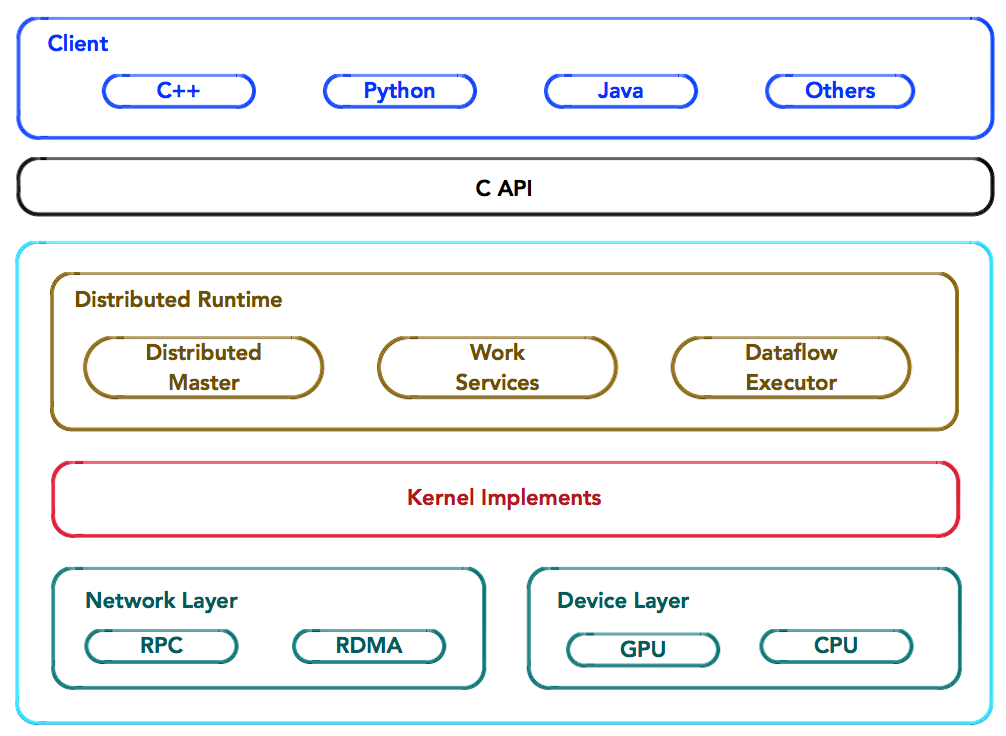
\includegraphics[width=0.7\textwidth]{framework.png}
  \end{figure}
\end{frame}

\begin{frame}{设计原则}
    \begin{itemize}
      \item \alert{延迟计算}:图的构造与执行分离,并推迟计算图的执行过程
      \item \alert{原子OP}:OP是最小的抽象计算单元,支持构造复杂的网络模型
      \item \alert{抽象设备}:支持CPU, GPU, ASIC多种异构设备类型
      \item \alert{抽象任务}:基于任务的PS,支持优化算法和网络模型的扩展
    \end{itemize}
\end{frame}

\subsection{图控制}

\begin{frame}{构造计算图}
  \begin{figure}
    \centering
    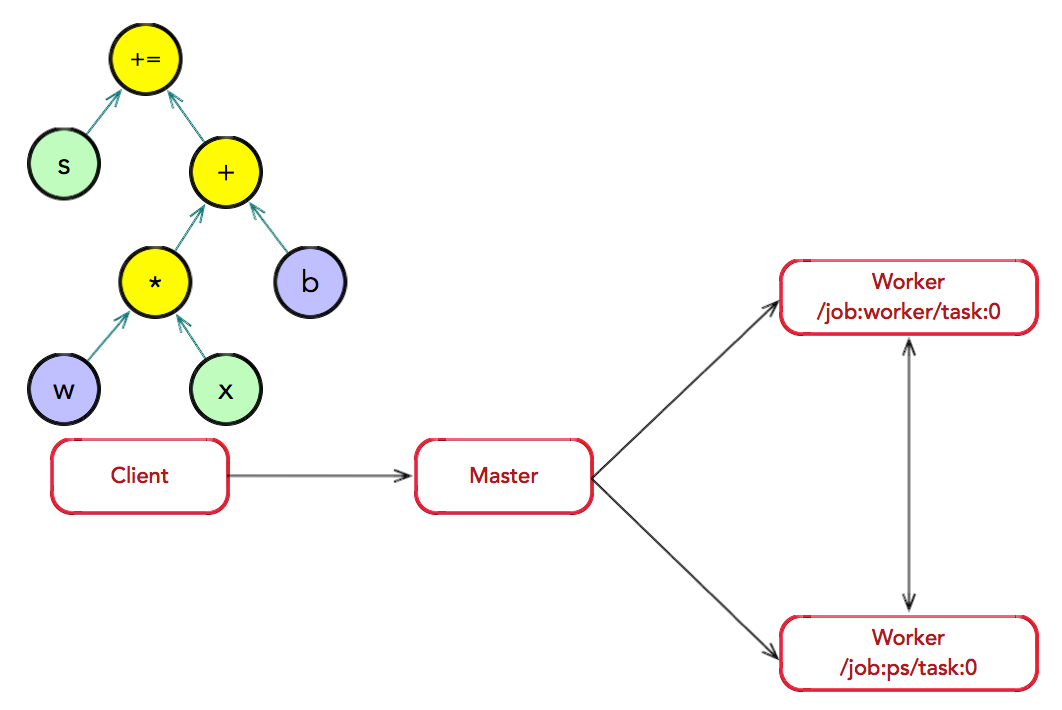
\includegraphics[width=0.75\textwidth]{construct-graph.png}
  \end{figure}
\end{frame}

\begin{frame}{执行计算图}
  \begin{figure}
    \centering
    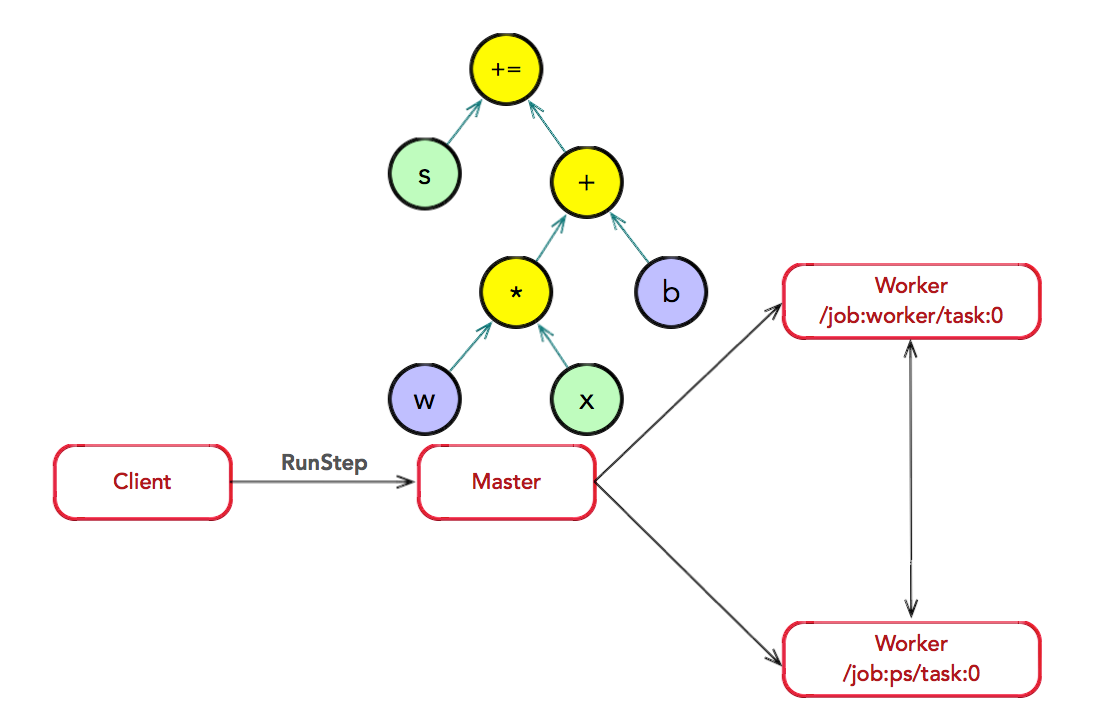
\includegraphics[width=0.8\textwidth]{execute-graph.png}
  \end{figure}
\end{frame}

\begin{frame}{图分解}
  \begin{figure}
    \centering
    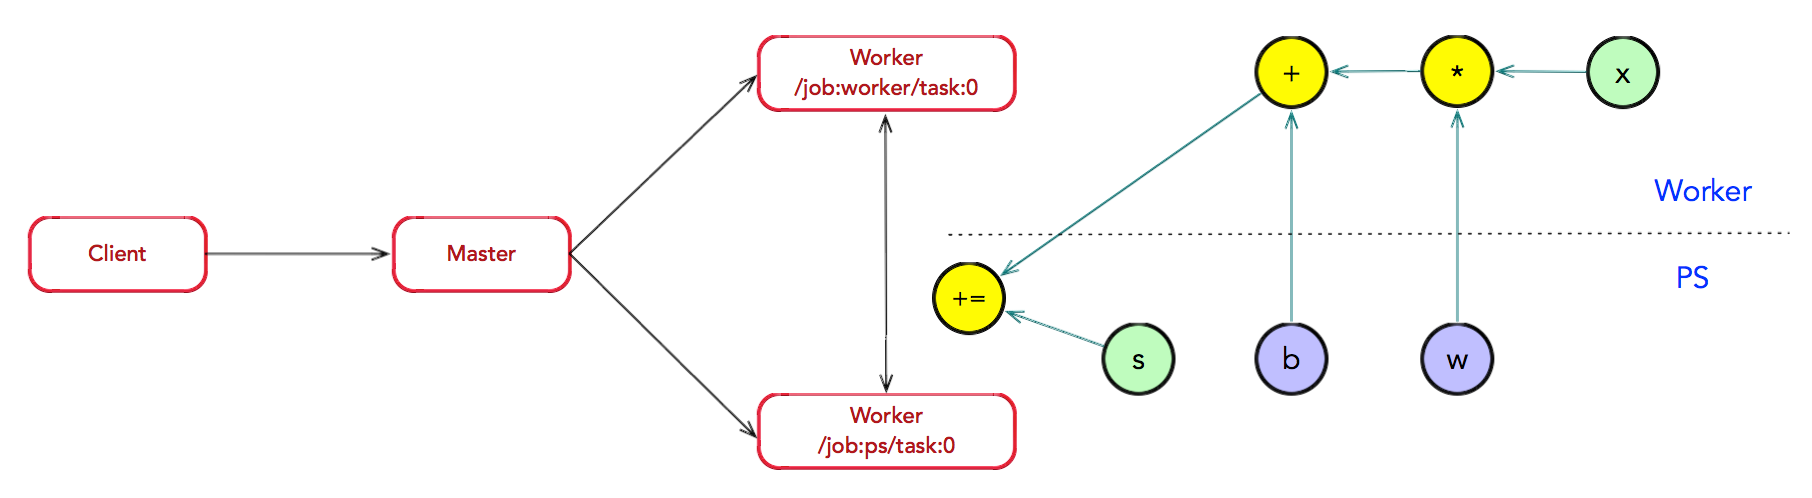
\includegraphics[width=1.0\textwidth]{split-graph-by-task.png}
  \end{figure}
\end{frame}

\begin{frame}{注册图}
  \begin{figure}
    \centering
    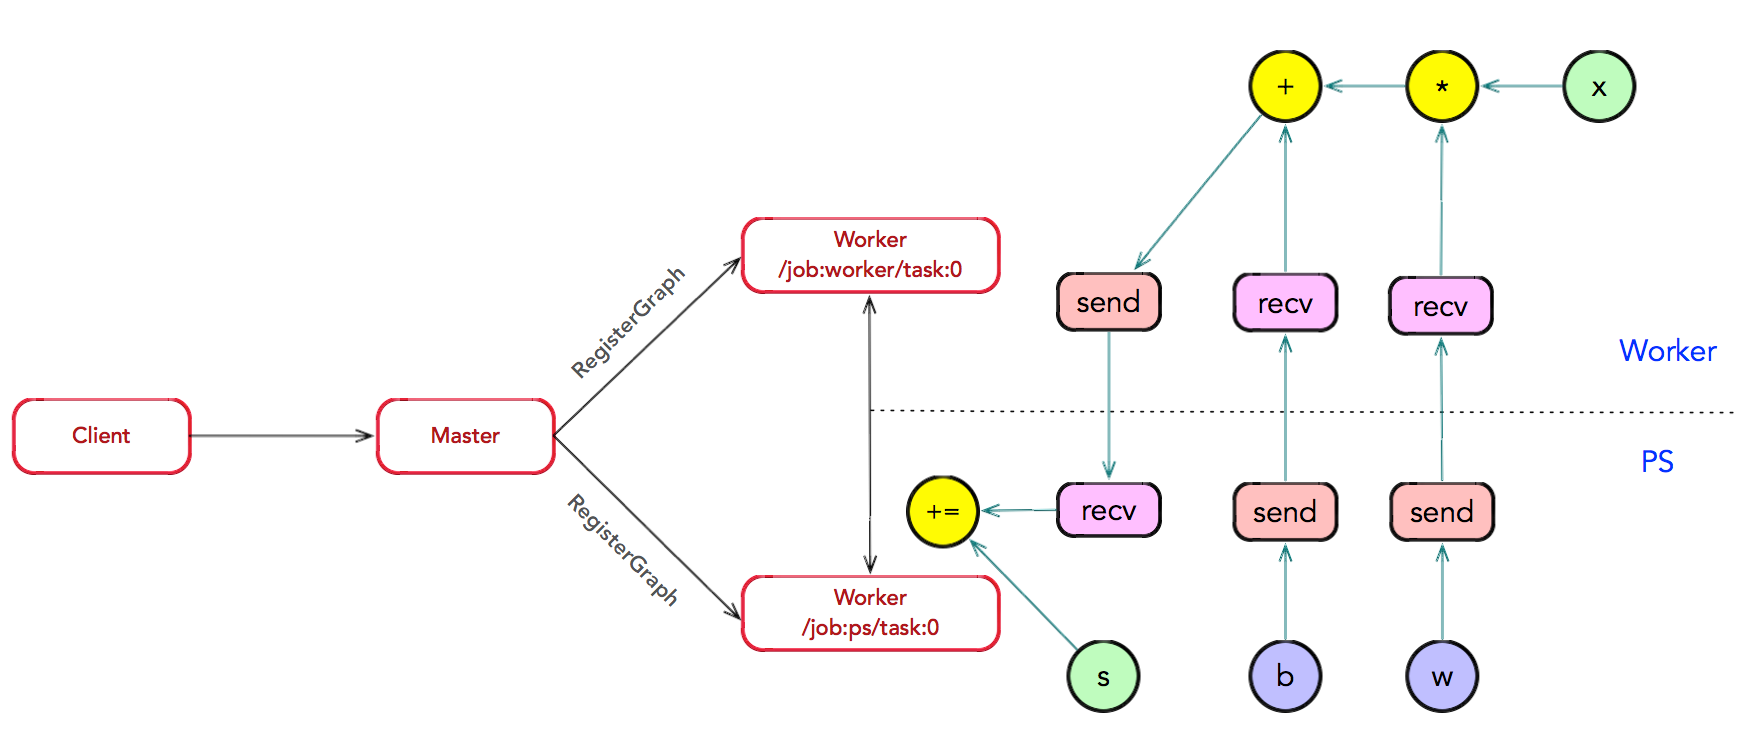
\includegraphics[width=1.0\textwidth]{register-graph.png}
  \end{figure}
\end{frame}

\begin{frame}{执行图}
  \begin{figure}
    \centering
    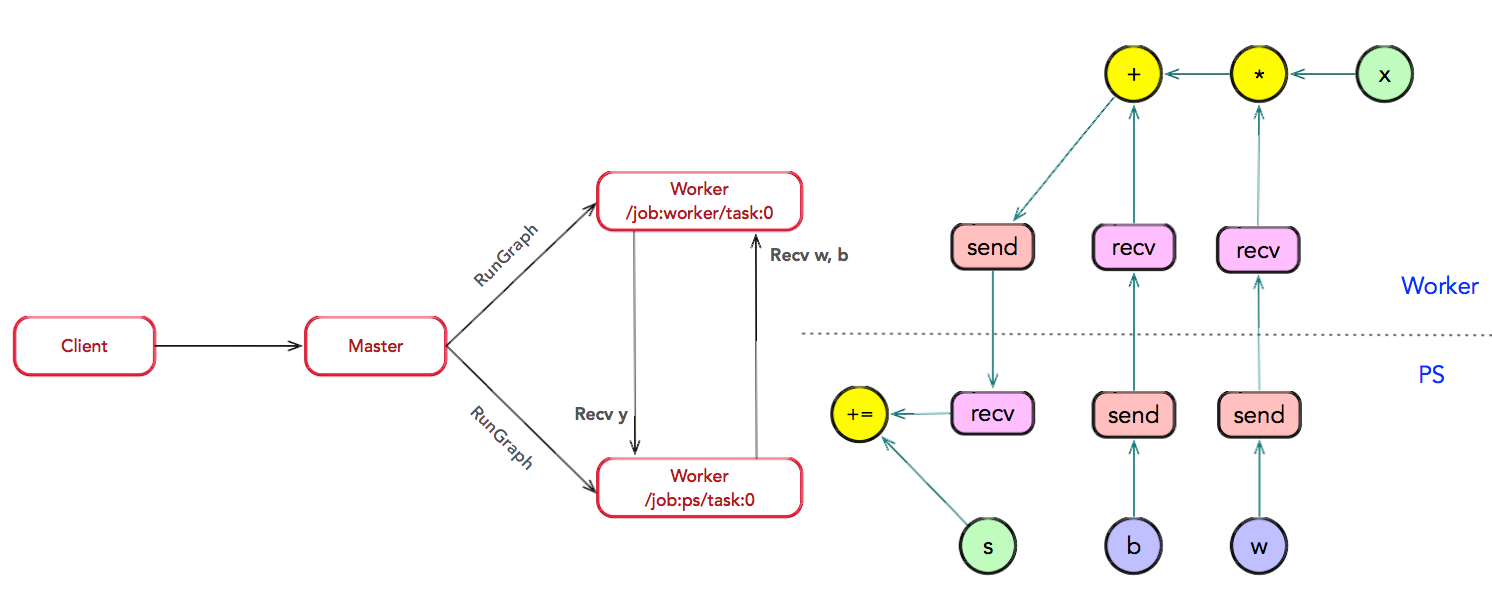
\includegraphics[width=1.0\textwidth]{run-graph.png}
  \end{figure}
\end{frame}

